\newcommand{\techniques}{

\part{Experimental Techniques}

\section{Scanning Electron Microscope}

The scanning electron microscope (SEM) is a widely used technique in materials science as a means to study the surface of materials in high resolution and, perhaps one of the most distinguishing features of the SEM, in high depth of field, giving the images a three dimensional appearance. \citep{Leng2013}
\begin{wrapfigure}{l}{0.5\textwidth}%\hspace*{-1.5cm}
\centering
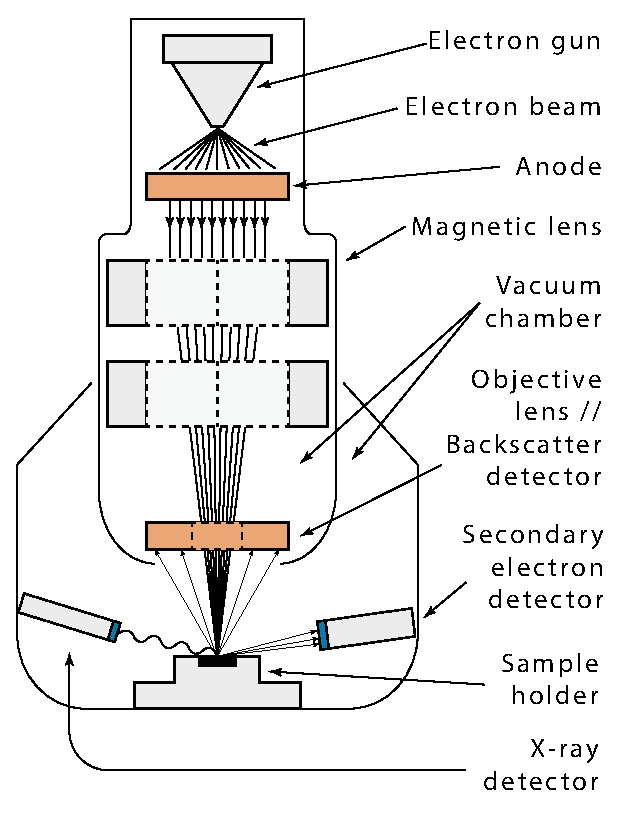
\includegraphics[scale=0.8]{Figures/SEM_schematic.eps}
\caption{\intextnote{Fill inn}}
\label{fig:SEM:schematic}
\end{wrapfigure}

As can be seen in figure \ref{fig:SEM:schematic} the SEM operates on the basis that an electron beam is produced by an electron gun, then concentrated and directed through a series of electric and magnetic lenses. The acceleration voltage in a SEM is typically in the range 1-40 kV and the number of lenses can vary from one to three, depending on the manufacturer. The first lenses are used to demagnify the beam and control the diameter of the beam while the last lens are use to focus the beam upon the sample. Apertures are also utilized to optimize the beam diameter, focal point and working distance to ensure a high quality image; these are usually placed right after the last lens, but are sometimes also used in between the lenses to enhance control of the electron beam.



Small probe diameter is favourable for high res. Probe diameter approx expressed as $d_p$
\begin{align*}
d_p \eq \para{
\dfrac{4i_p}{\beta \pi^2\alpha_\text{f}^2}
}^{1/2}
\end{align*}
where $i_p$ is the probe current, $\beta$ is the beam brightness. Regardless of e-source type the brightness is proportional to the acceleration voltage $V_{\text{o}}$ via 
\begin{align*}
\beta\propto e V_{\text{o}}
\end{align*}
and $\alpha_{\text{f}}$ is the convergence angle of the probe. 

Obtain minimal probe size by increasing the brightness as ewll as the convergence angle. $\alpha_{\text{f}}$ is likely to cause optical problems at large values and must therefore be optimized not simply increased. With an optimized $\alpha_{\text{f}}$ the minimum probe size is approximated as $d_{min}$
\begin{align*}
d_{\text{min}}\eq KC_s^{1/4}\para{\dfrac{i_p}{\beta}+\lambda^2}^{3/8}
\end{align*}
$K$ is a constant close to unity, $C_s$ is the sphreical aberration coefficient and $\lambda$ is the wavelength of the electrons. 






}